\documentclass[conference]{IEEEtran}

\usepackage[utf8]{inputenc}
\usepackage[T1]{fontenc}
\usepackage{amsmath,amssymb}
\usepackage{graphicx}
\usepackage{subcaption}
\usepackage{booktabs}
\usepackage{hyperref}
\usepackage{algorithm}
\usepackage{algpseudocode}
\usepackage{xcolor}
\usepackage{float}

\graphicspath{{docs/images/}{docs/output/}}

\title{Image Denoising: A Comparative Study of Classical Signal Processing Methods}

\author{
  \IEEEauthorblockN{[Alexandru-Ionuț Țîncu]}
  \IEEEauthorblockA{
    Facultatea de Matematică și Informatică \\
    Universitatea din București \\
    București, România \\
  }
}

\begin{document}

\maketitle

% ─────────────────────────────────────────────────────────────────────────────
\begin{abstract}
Image denoising is the problem of recovering a clean image from a corrupted photograph, where the corruption arises from noise introduced during capture, transmission, or storage. This paper investigates five classical signal processing methods for image denoising: Gaussian filtering, bilateral filtering, Fourier-domain low-pass filtering, wavelet thresholding, and median filtering. Each method is implemented from scratch using NumPy and SciPy, and evaluated on two canonical noise models: additive white Gaussian noise (AWGN)
and salt-and-pepper impulse noise. Performance is measured using Peak Signal-to-Noise Ratio (PSNR) and the Structural Similarity Index (SSIM).

Results show that bilateral filtering achieves the highest PSNR of 27.25 dB under Gaussian noise while preserving edges, whereas median filter is the most effective filtering against salt-and-pepper noise, achieving 28.16 dB PSNR.
\end{abstract}

% ─────────────────────────────────────────────────────────────────────────────
\section{Introduction}

Digital images are inevitably degraded by noise during their acquisition and processing pipeline. Sensor thermal noise, photon shot noise, quantization errors, and transmission channel errors all manifest as unwanted random variation superimposed on the true image signal. Removing this noise while preserving the perceptually important structures in the image, primarily edges and fine textures, is one of the central problems in image processing.

The problem is relevant beyond purely academic interest. In medical imaging, noise reduction directly affects diagnostic accuracy: a blurred or artifact-laden MRI or CT scan can obscure pathologies and lead to incorrect clinical decisions. In remote sensing and satellite imagery, denoising is a prerequisite for any downstream analysis such as segmentation or change detection. In consumer photography, real-time denoising pipelines are embedded in every modern smartphone ISP (Image Signal Processor).

Formally, the degradation model is:

\begin{equation}
  \mathbf{y} = \mathbf{x} + \mathbf{n}
  \label{eq:degradation}
\end{equation}

where $\mathbf{x} \in \mathbb{R}^{H \times W}$ is the latent clean image, $\mathbf{n}$ is a noise process, and $\mathbf{y}$ is the observed noisy image. The goal is to recover an estimate $\hat{\mathbf{x}}$ of $\mathbf{x}$ from $\mathbf{y}$ alone.

The methods studied in this work span three families of classical approaches: (1) spatial-domain filtering (Gaussian and bilateral), which operate directly on pixel neighborhoods; (2) transform-domain filtering (Fourier and wavelet), which exploit the sparsity of natural images in a transformed basis; and (3) nonlinear order-statistics filtering (median), which is robust to impulsive noise.

Classical denoising methods have found success in many practical settings. Bilateral filtering is widely used in real-time rendering pipelines and computational photography. Wavelet-based methods underpin the JPEG 2000 compression standard and are used in medical image archiving. Median filtering remains the standard preprocessing step for removing impulse noise in embedded vision systems due to its simplicity and hardware efficiency.

% ─────────────────────────────────────────────────────────────────────────────
\section{State of the Art}

\subsection{Spatial Filtering}

The simplest approach to noise reduction is convolving the image with a low-pass kernel. The Gaussian filter replaces each pixel with a weighted average of its neighborhood, where weights follow a 2D Gaussian distribution:
    
\begin{equation}
  k_G(i,j) = \frac{1}{2\pi\sigma^2} \exp\!\left(-\frac{i^2 + j^2}{2\sigma^2}\right)
  \label{eq:gaussian_kernel}
\end{equation}

The filtered image is obtained via convolution: $\hat{x}[i,j] = (k_G * y)[i,j]$. While computationally efficient, Gaussian filtering is a linear operation and treats signal and noise indiscriminately at the same spatial scale, inevitably blurring edges.

The bilateral filter, introduced by Tomasi and Manduchi, addresses this by adding a second, intensity-domain weight to the averaging:

\begin{equation}
  \hat{x}[i,j] = \frac{1}{W_{ij}} \sum_{(k,l) \in \mathcal{N}}
    G_s(k,l) \cdot G_r\!\left(y[i+k,j+l] - y[i,j]\right) \cdot y[i+k,j+l]
  \label{eq:bilateral}
\end{equation}

where $G_s$ is the spatial Gaussian with standard deviation $\sigma_s$, $G_r$ is the range Gaussian with standard deviation $\sigma_r$, and $W_{ij}$ is a normalizing factor. Pixels across a sharp intensity edge have a large intensity difference and therefore a small range weight, so they contribute negligibly to the output. This makes the bilateral filter edge-preserving by construction.

\subsection{Fourier-Domain Filtering}

In the frequency domain, AWGN has a flat power spectral density: noise energy is distributed uniformly across all frequencies. Natural images, by contrast, follow a $1/f^2$ power spectrum and concentrate most of their energy at low frequencies. A circular low-pass filter in the Fourier domain retains this low-frequency signal while suppressing the high-frequency noise:

\begin{equation}
  \hat{X}(u,v) = X(u,v) \cdot M(u,v), \quad
  M(u,v) = \begin{cases} 1 & u^2 + v^2 \leq r^2 \\ 0 & \text{otherwise} \end{cases}
  \label{eq:fourier_lpf}
\end{equation}

The filtered image is recovered as $\hat{x} = \mathcal{F}^{-1}\{\hat{X}\}$. The cutoff radius $r$ is expressed as a fraction of the image dimension and is the single free parameter of the method. A binary mask produces Gibbs ringing artifacts; apodized (windowed) variants can mitigate this but are not implemented here for simplicity.

\subsection{Wavelet Thresholding}

Wavelet thresholding, formalized by Donoho and Johnstone, rests on the observation that natural images have a sparse representation in wavelet bases: most energy is concentrated in a small number of large-magnitude coefficients, whereas AWGN projects uniformly onto all basis functions. Denoising proceeds by decomposing the noisy image, thresholding the detail coefficients, and reconstructing:

\begin{align}
  \mathbf{C} &= \mathcal{W}\{\mathbf{y}\} \label{eq:wt_forward} \\
  \tilde{C}_{j,k} &= \mathcal{T}_\lambda(C_{j,k}) \label{eq:wt_threshold} \\
  \hat{\mathbf{x}} &= \mathcal{W}^{-1}\{\tilde{\mathbf{C}}\} \label{eq:wt_inverse}
\end{align}

where $\mathcal{W}$ denotes the discrete wavelet transform (DWT) and $\mathcal{T}_\lambda$ is a thresholding operator. Two common choices are:

\begin{align}
  \mathcal{T}^{\text{hard}}_\lambda(c) &= c \cdot \mathbf{1}[|c| > \lambda]
  \label{eq:hard_thresh} \\
  \mathcal{T}^{\text{soft}}_\lambda(c) &= \text{sgn}(c) \cdot \max(|c| - \lambda, 0)
  \label{eq:soft_thresh}
\end{align}

The VisuShrink threshold is derived from extreme value theory and set to:

\begin{equation}
  \lambda = \hat{\sigma} \sqrt{2 \log N}
  \label{eq:visushrink}
\end{equation}

where $N$ is the number of pixels and $\hat{\sigma}$ is estimated from the finest-scale detail coefficients via the robust estimator:

\begin{equation}
  \hat{\sigma} = \frac{\text{median}(|C_{\text{detail}}|)}{0.6745}
  \label{eq:sigma_est}
\end{equation}

\subsection{Median Filtering}

The median filter replaces each pixel with the median of the values in a
$(2k+1) \times (2k+1)$ neighborhood:

\begin{equation}
  \hat{x}[i,j] = \text{median}\!\left\{ y[i+k, j+l] : (k,l) \in \mathcal{N} \right\}
  \label{eq:median}
\end{equation}

It is a nonlinear filter with no closed-form frequency response, but its key property is robustness to impulse noise: a single extreme value (0 or 255) cannot survive the median operation when surrounded by pixels in a normal intensity range. The median filter was introduced to image processing by Tukey and is optimal in an $L_1$ sense for symmetric noise distributions.
    
\subsection{Modern Deep Learning Methods}

For completeness, recent state-of-the-art methods are based on convolutional neural networks trained on large image corpora. DnCNN uses residual learning to predict the noise component directly. FFDNet extends this to handle spatially varying noise levels via a noise-level map input. Blind-spot networks such as Noise2Void and Noise2Self remove the requirement for clean training data entirely. These methods consistently outperform classical approaches in PSNR by 2--5 dB on standard benchmarks but require GPU infrastructure and large datasets; classical methods remain preferred in resource-constrained or interpretability-critical settings.

% ─────────────────────────────────────────────────────────────────────────────
\section{Methods}

This section describes the five denoising methods implemented in this work, with attention to the algorithmic steps and their computational complexity.

\subsection{Gaussian Filter}

The 2D Gaussian kernel of size $(2m+1) \times (2m+1)$ with parameter $\sigma$ is constructed analytically according to and normalized so that its coefficients sum to one. The image is zero-padded (reflect mode) and convolved with the kernel using a direct sliding-window implementation. For a color image, each channel is convolved independently.

\begin{algorithm}
\caption{Gaussian Filter}
\begin{algorithmic}[1]
\Require Noisy image $\mathbf{y}$, kernel size $m$, parameter $\sigma$
\State Build kernel $k_G$ via \eqref{eq:gaussian_kernel}; normalize: $k_G \leftarrow k_G / \sum k_G$
\State Pad $\mathbf{y}$ with $m$ rows/columns using reflect padding
\For{each pixel $(i,j)$}
  \State $\hat{x}[i,j] \leftarrow \sum_{(k,l)} k_G[k,l] \cdot y_{\text{pad}}[i+k, j+l]$
\EndFor
\State \Return $\hat{\mathbf{x}}$
\end{algorithmic}
\end{algorithm}

\textbf{Complexity.} For an $H \times W$ image and kernel of size $K \times K$, the naive implementation runs in $O(HW K^2)$. Using separability of the Gaussian kernel, this reduces to $O(HWK)$ with two 1D passes; the FFT-based convolution achieves $O(HW \log(HW))$ regardless of kernel size.

\subsection{Bilateral Filter}

The bilateral filter iterates over every pixel and over every neighbor within the window, computing the product of spatial and range weights.

\begin{algorithm}
\caption{Bilateral Filter}
\begin{algorithmic}[1]
\Require Noisy image $\mathbf{y}$, window size $m$, $\sigma_s$, $\sigma_r$
\State Precompute spatial weights: $G_s[k,l] = \exp(-(k^2+l^2)/(2\sigma_s^2))$
\State Pad $\mathbf{y}$ with $m$ rows/columns
\For{each pixel $(i,j)$}
  \State Extract patch $P \leftarrow y_{\text{pad}}[i:i+2m+1, j:j+2m+1]$
  \State $G_r \leftarrow \exp(-(P - P_{\text{center}})^2 / (2\sigma_r^2))$
  \State $W \leftarrow G_s \odot G_r$ \Comment{element-wise product}
  \State $\hat{x}[i,j] \leftarrow \sum(W \odot P) / \sum(W)$
\EndFor
\State \Return $\hat{\mathbf{x}}$
\end{algorithmic}
\end{algorithm}

\textbf{Complexity.} $O(HW K^2)$ with $K = 2m+1$. The spatial weights are precomputed once. The range weights must be recomputed per pixel because they depend on the center pixel value. This makes the bilateral filter significantly more expensive than Gaussian filtering for the same window size; approximate methods such as the fast bilateral filter reduce this to near-linear time.

\subsection{Fourier Low-Pass Filter}

The 2D FFT is computed, shifted so that the DC component is at the center, and masked with a binary circle. The inverse FFT then recovers the filtered image.

\begin{algorithm}
\caption{Fourier Low-Pass Filter}
\begin{algorithmic}[1]
\Require Noisy image channel $y$, cutoff fraction $\rho \in (0,1)$
\State $F \leftarrow \mathcal{F}\{y\}$; shift DC to center
\State $r \leftarrow \rho \cdot \min(H, W)$
\State Build binary mask $M$: $M[u,v] = 1$ iff $(u-H/2)^2 + (v-W/2)^2 \leq r^2$
\State $\hat{X} \leftarrow F \odot M$
\State $\hat{x} \leftarrow \Re\{\mathcal{F}^{-1}\{\text{shift back}(\hat{X})\}\}$
\State \Return $\text{clip}(\hat{x}, 0, 255)$
\end{algorithmic}
\end{algorithm}

\textbf{Complexity.} $O(HW \log(HW))$ for the FFT and inverse FFT; mask construction is $O(HW)$.

\subsection{Wavelet Thresholding}

A multilevel 2D DWT using the Daubechies-4 (db4) wavelet is applied to the noisy image. The noise standard deviation is estimated from the finest-scale horizontal detail subband. The VisuShrink threshold is computed and soft thresholding is applied to all detail subbands. The approximation subband is left untouched.

\begin{algorithm}
\caption{Wavelet Soft Thresholding (VisuShrink)}
\begin{algorithmic}[1]
\Require Noisy image channel $y$, wavelet $\psi$, levels $L$
\State $\mathbf{C} \leftarrow \text{wavedec2}(y, \psi, L)$
\State Collect all detail coefficients $\{C_{j,k}\}_{j=1}^{L}$
\State $\hat{\sigma} \leftarrow \text{median}(|\{C_{j,k}\}|) / 0.6745$
\State $\lambda \leftarrow \hat{\sigma}\sqrt{2\log N}$, where $N = HW$
\For{each detail subband at each level}
  \State $\tilde{C} \leftarrow \text{sgn}(C) \cdot \max(|C| - \lambda,\ 0)$
\EndFor
\State $\hat{x} \leftarrow \text{waverec2}(\{\tilde{\mathbf{C}}\}, \psi)$
\State \Return $\text{clip}(\hat{x}[:H, :W], 0, 255)$
\end{algorithmic}
\end{algorithm}

\textbf{Complexity.} The DWT at level $L$ costs $O(HW)$ per level using filter-bank subsampling, giving $O(LHW)$ total. The thresholding step is $O(HW)$.

\subsection{Median Filter}

Each pixel is replaced by the median of its $K \times K$ neighborhood.

\begin{algorithm}
\caption{Median Filter}
\begin{algorithmic}[1]
\Require Noisy image channel $y$, window size $K$
\State $m \leftarrow K // 2$; pad $y$ with $m$ rows/columns (reflect mode)
\For{each pixel $(i,j)$}
  \State $\hat{x}[i,j] \leftarrow \text{median}(y_{\text{pad}}[i:i+K, j:j+K])$
\EndFor
\State \Return $\hat{\mathbf{x}}$
\end{algorithmic}
\end{algorithm}

\textbf{Complexity.} $O(HW K^2 \log K)$ using comparison-based sorting per window. Histogram-based constant-time median filters achieve $O(HW)$ but are not implemented here.

\subsection{Quality Metrics}

Two metrics are used throughout. PSNR (Peak Signal-to-Noise Ratio) measures the ratio between the maximum possible signal power and the mean squared error:

\begin{equation}
  \text{PSNR}(\mathbf{x}, \hat{\mathbf{x}}) =
    10 \log_{10}\!\left(\frac{255^2}{\text{MSE}(\mathbf{x}, \hat{\mathbf{x}})}\right)
  \label{eq:psnr}
\end{equation}

SSIM (Structural Similarity Index) measures perceptual similarity along three dimensions: luminance, contrast, and structure:

\begin{equation}
  \text{SSIM}(\mathbf{x}, \hat{\mathbf{x}}) =
    \frac{(2\mu_x \mu_{\hat{x}} + C_1)(2\sigma_{x\hat{x}} + C_2)}
         {(\mu_x^2 + \mu_{\hat{x}}^2 + C_1)(\sigma_x^2 + \sigma_{\hat{x}}^2 + C_2)}
  \label{eq:ssim}
\end{equation}

where $\mu$, $\sigma^2$, and $\sigma_{x\hat{x}}$ denote means, variances, and cross-covariance; $C_1 = (0.01 \cdot 255)^2$ and $C_2 = (0.03 \cdot 255)^2$are stabilizing constants.

% ─────────────────────────────────────────────────────────────────────────────
\section{Implementation}

\subsection{Libraries and Frameworks}

The implementation uses Python 3 with the following libraries:

\begin{itemize}
  \item \textbf{NumPy} for all array operations, kernel construction, and
    sliding-window loops.
  \item \textbf{SciPy} (\texttt{scipy.fft}) for the 2D FFT and inverse FFT.
    SciPy's FFT implementation uses the Cooley-Tukey algorithm with FFTPACK
    as backend.
  \item \textbf{PyWavelets} for the multilevel 2D DWT and inverse DWT, and for
    the soft/hard thresholding operator.
  \item \textbf{Pillow} for image I/O.
  \item \textbf{Matplotlib} for visualization.
\end{itemize}

No high-level denoising functions from scikit-image are used; all filterimplementations are written from scratch using NumPy array primitives.

\subsection{Data Structures}

Images are represented as NumPy arrays of shape $(H, W, 3)$ with dtype \texttt{float64} during processing to avoid integer overflow in intermediate computations. The final output is clipped to $[0, 255]$ and cast to \texttt{uint8} before saving. Grayscale conversion for metric computation is performed by averaging the three color channels.

Wavelet coefficients are stored as a list of tuples in PyWavelets' native format: \texttt{[approx, (H1, V1, D1), (H2, V2, D2), \ldots]}, where each tuple contains horizontal, vertical, and diagonal detail subbands at one scale.

\subsection{Color Image Handling}

All five methods process color images by applying the filter independently to each RGB channel and stacking the results. While this is not optimal for all color spaces (e.g., chrominance channels could be treated differently), it is the standard approach for classical spatial filters and preserves compatibility with the grayscale metric computation.

\subsection{Parallelism}

The current implementation is single-threaded. The per-pixel loops in the Gaussian, bilateral, and median filters are the primary bottleneck. Each pixel can be processed independently, making these loops embarrassingly parallel. A straightforward optimization would be to use NumPy's vectorized operations with \texttt{np.lib.stride\_tricks.sliding\_window\_view} for the Gaussian and median filters. The bilateral filter's per-pixel range weight computation resists simple vectorization but can be parallelized across pixels using Python's \texttt{multiprocessing} module or Numba's JIT compiler.

% ─────────────────────────────────────────────────────────────────────────────
\section{Experiments}

\subsection{Experimental Setup}

Experiments are conducted on the photograph of Mount Everest found on the Wikipedia "Mountain" page, of a size of 2000x1333 pixels. The picture was taken by Luca Galuzzi on the 18th of August 2006, with the description "Mount Everest North Face as seen from the path to the base camp, Rongbuk Valley, Tibet (5,160 m).".

Two noise conditions are evaluated:
\begin{itemize}
  \item Additive White Gaussian Noise (AWGN) with $\sigma = 30$.
  \item Salt-and-pepper impulse noise with corruption probability $p = 0.05$.
\end{itemize}

The denoising parameters used are summarized in Table~\ref{tab:params}.

\begin{table}[h]
\centering
\caption{Denoising method parameters}
\label{tab:params}
\begin{tabular}{ll}
\toprule
Method & Parameters \\
\midrule
Gaussian filter & $\sigma = 2.0$, kernel size $7 \times 7$ \\
Bilateral filter & $\sigma_s = 5$, $\sigma_r = 30$, window $9 \times 9$ \\
Fourier LP filter & cutoff ratio $\rho = 0.15$ \\
Wavelet (soft) & db4 wavelet, $L = 3$ levels \\
Median filter & window $3 \times 3$ \\
\bottomrule
\end{tabular}
\end{table}

\subsection{Qualitative Results}

Figure~\ref{fig:gaussian_results} shows the visual output of all four methods under Gaussian noise on the Mountain image. Figure~\ref{fig:sp_results} shows results under salt-and-pepper noise.

\begin{figure}[H]
  \centering
  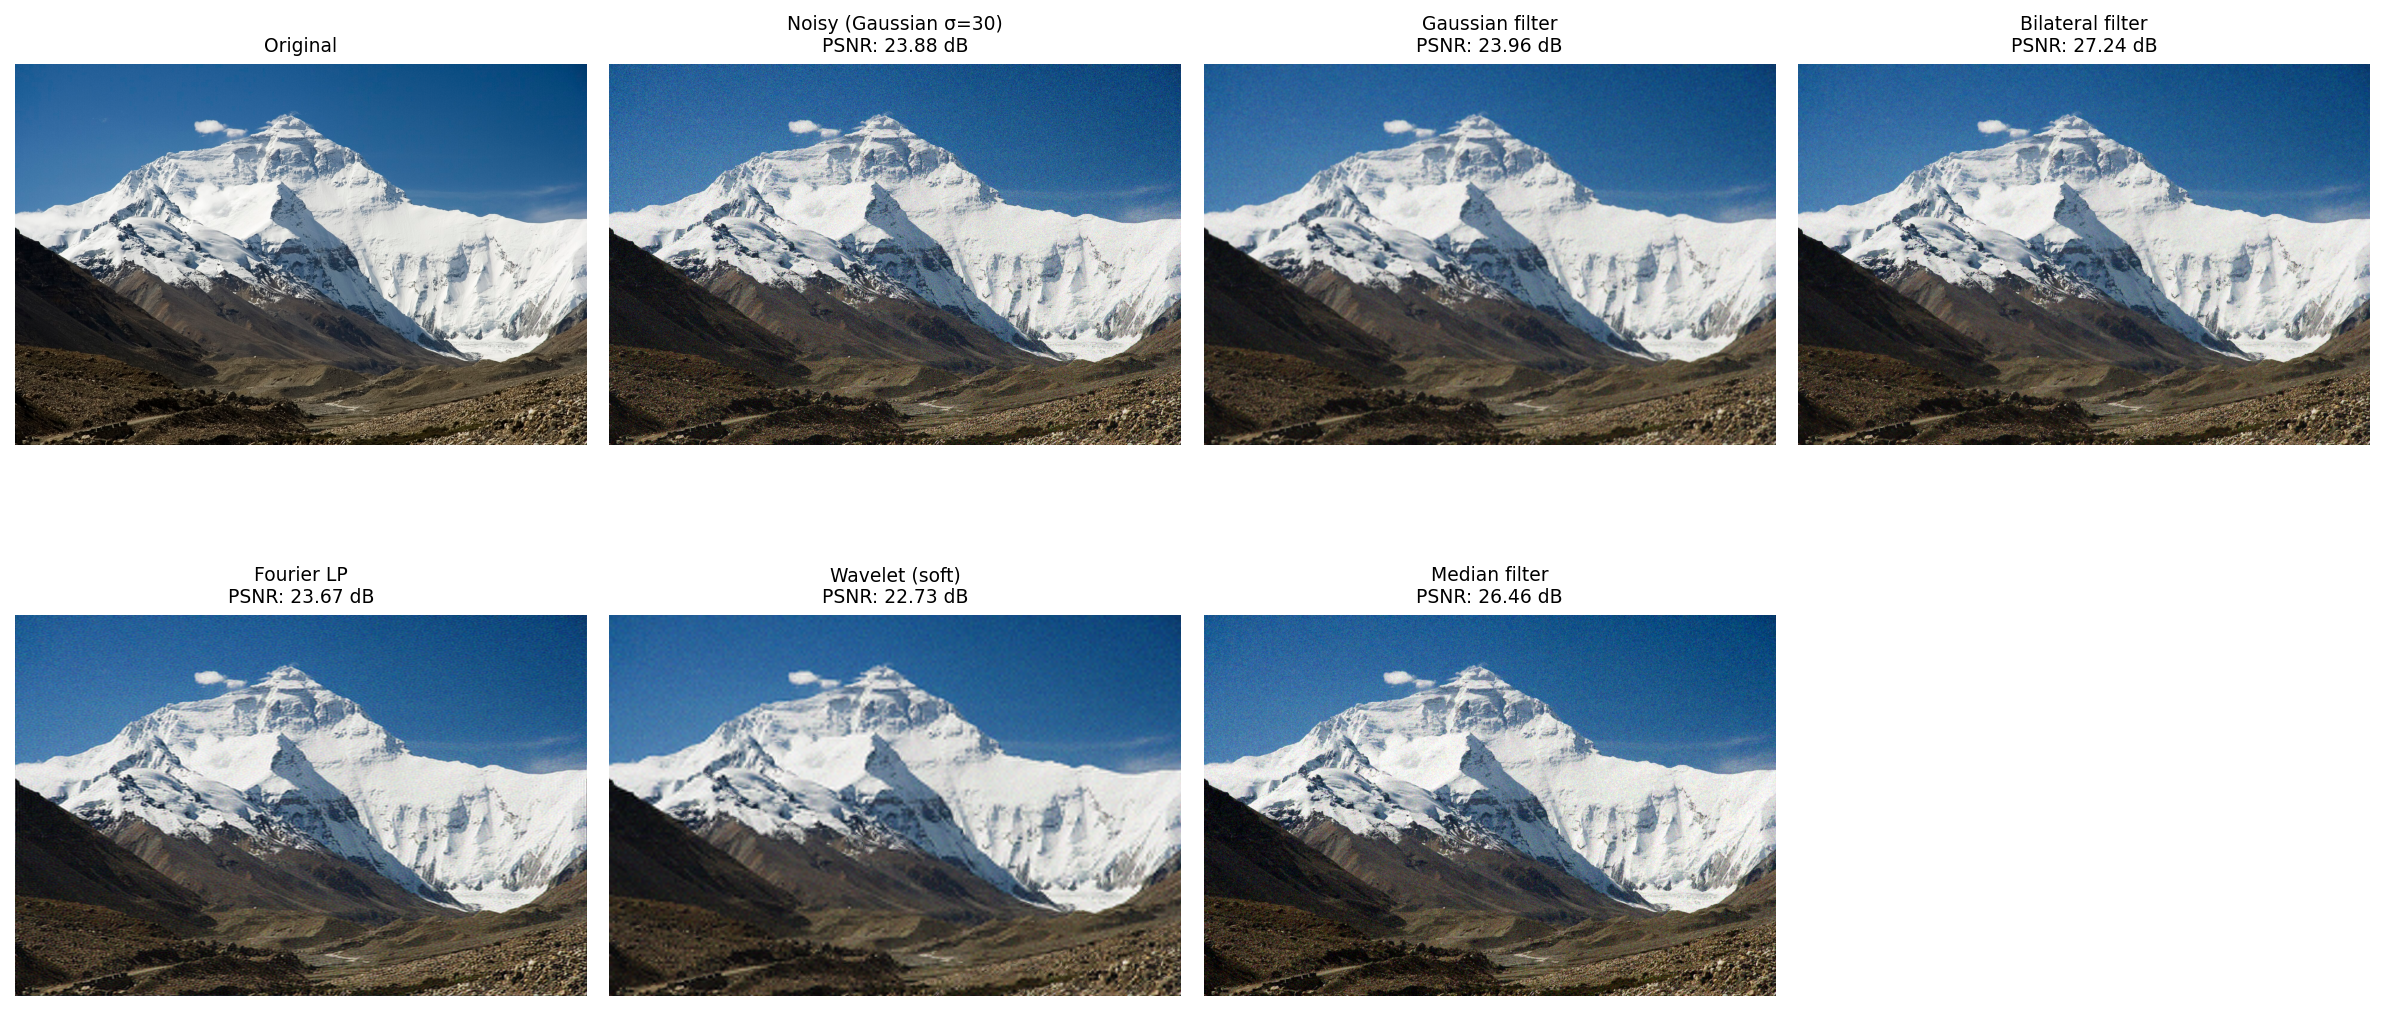
\includegraphics[width=\linewidth]{gaussian_noise_results.png}
  \caption{Denoising results under AWGN ($\sigma=30$). From left: original,
           noisy input, Gaussian filter, bilateral filter, Fourier LP, wavelet
           (soft thresholding). PSNR values are shown above each result.}
  \label{fig:gaussian_results}
\end{figure}

\begin{figure}[H]
  \centering
  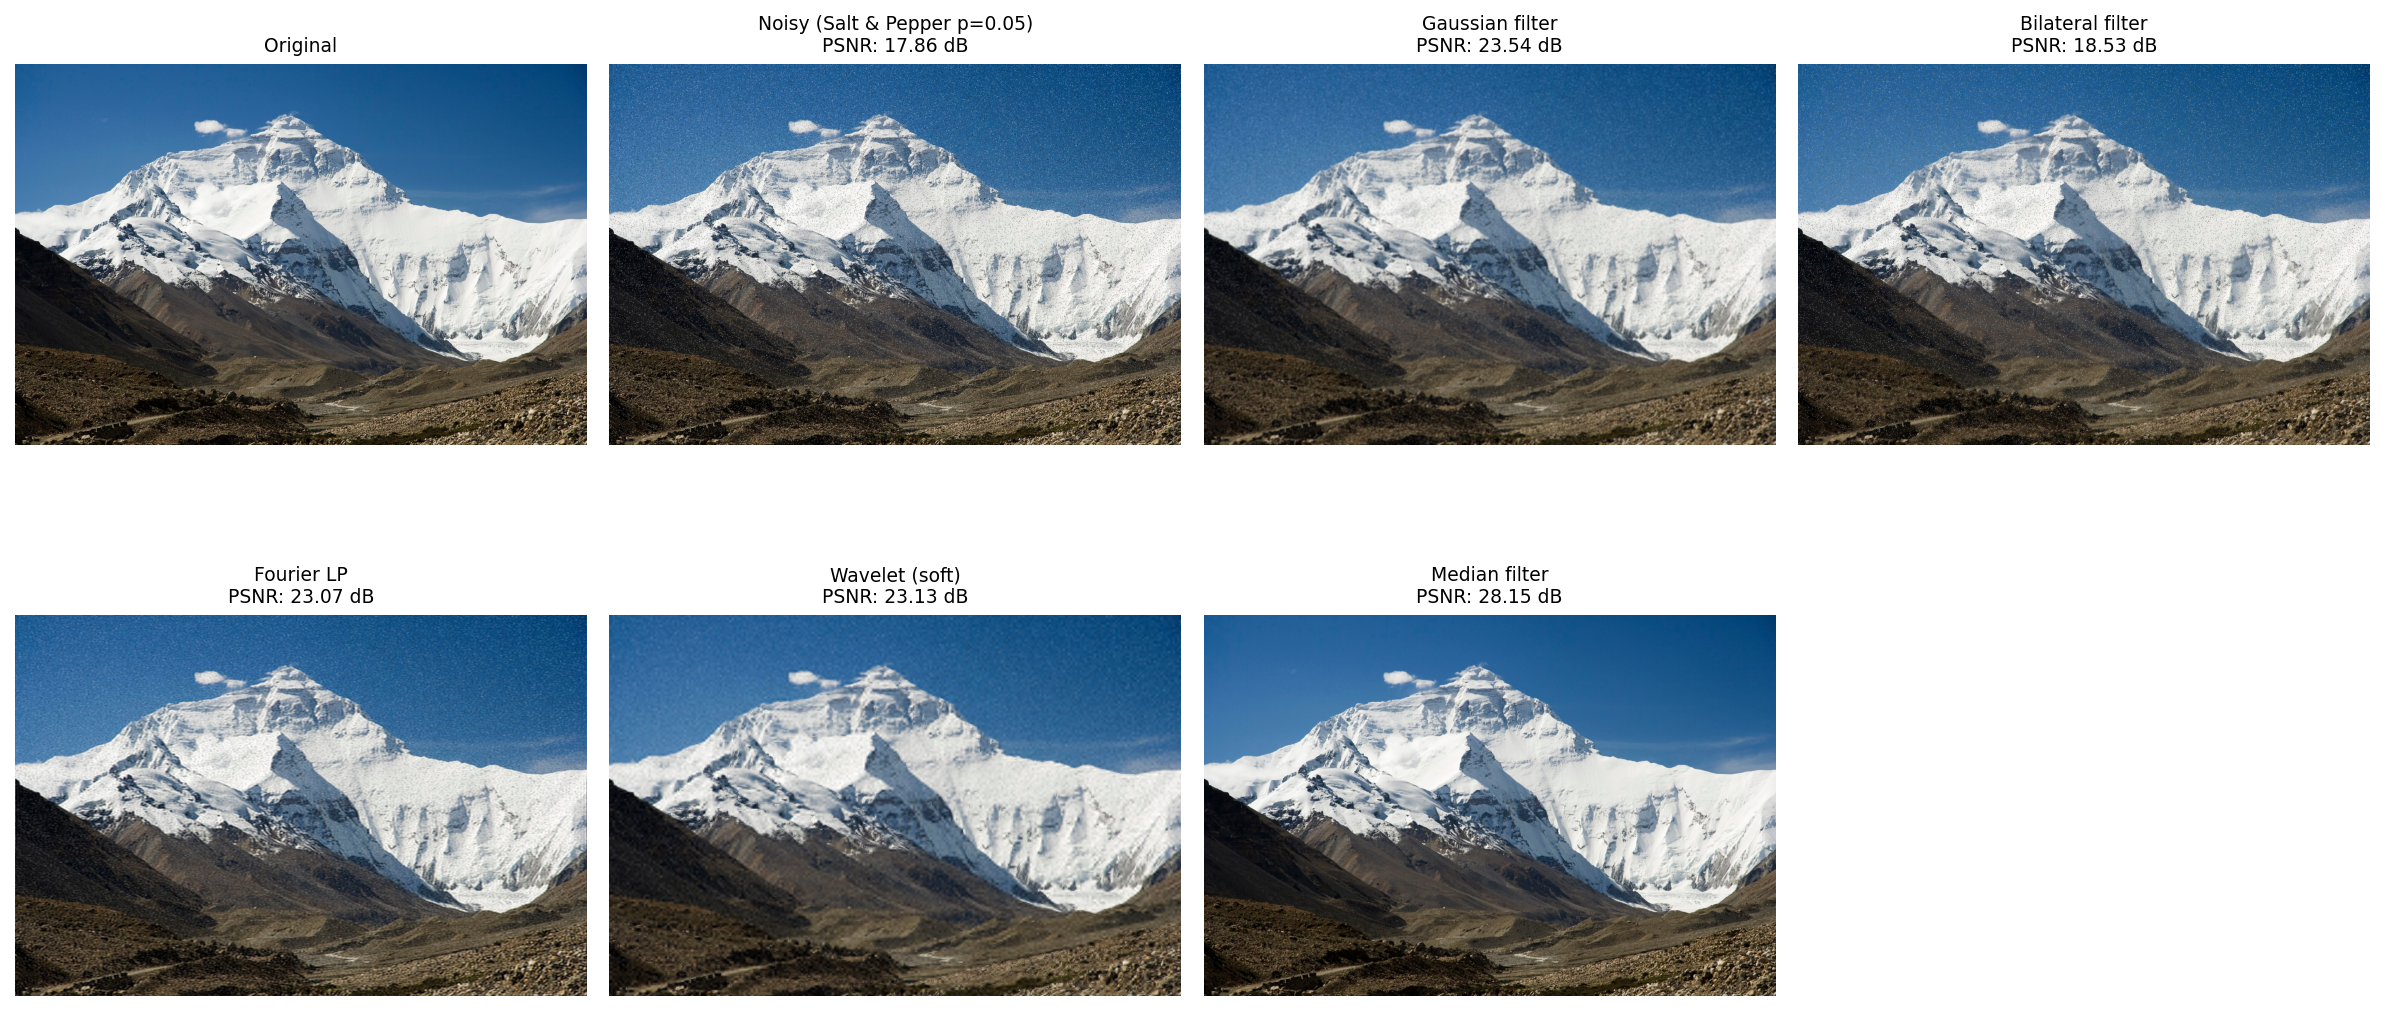
\includegraphics[width=\linewidth]{saltpepper_noise_results.png}
  \caption{Denoising results under salt-and-pepper noise ($p=0.05$). From left:
           original, noisy input, Gaussian filter, median filter, bilateral
           filter, wavelet (soft thresholding).}
  \label{fig:sp_results}
\end{figure}

\subsection{Fourier Spectrum Analysis}

Figure~\ref{fig:fourier_spectrum} shows the log-magnitude Fourier spectrum of the original, noisy, and Fourier-filtered images. Gaussian noise raises the energy floor uniformly across all frequencies; the low-pass mask zeros theouter ring of the spectrum, recovering the low-frequency image structure.

\begin{figure}[H]
  \centering
  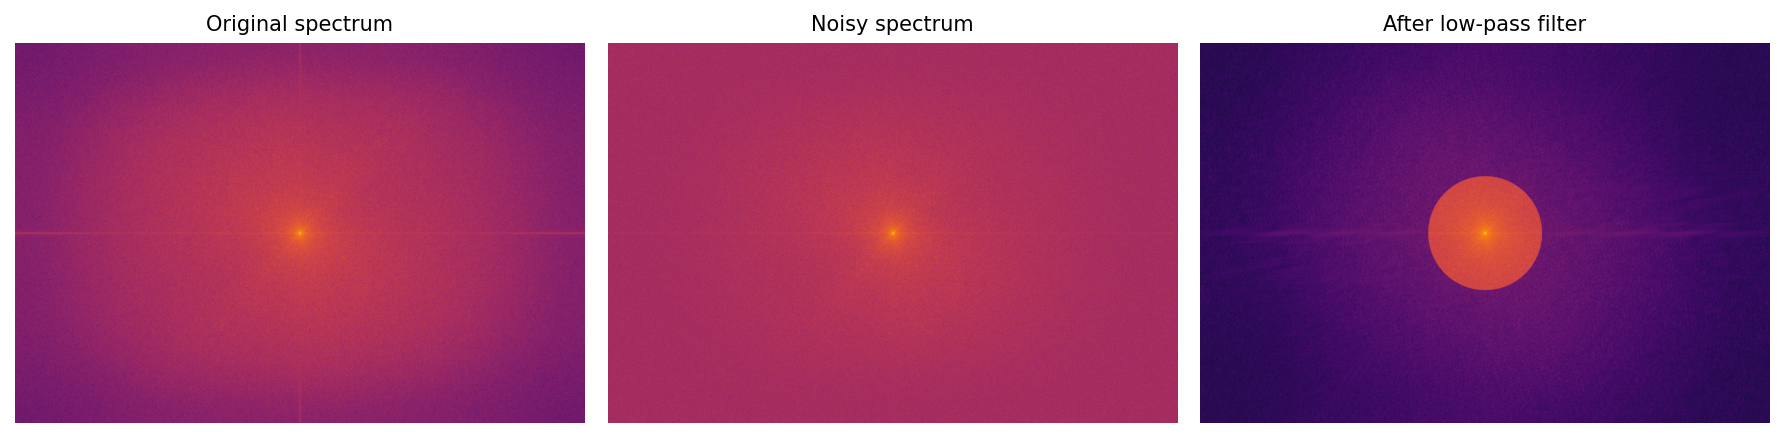
\includegraphics[width=\linewidth]{fourier_spectrum.png}
  \caption{Log-magnitude Fourier spectra. Left: original image spectrum showing
           energy concentration near the DC component. Center: spectrum of the
           noisy image, where AWGN raises the high-frequency floor. Right: after
           applying the circular low-pass mask.}
  \label{fig:fourier_spectrum}
\end{figure}

\subsection{Wavelet Coefficient Map}

Figure~\ref{fig:wavelet_coeffs} shows the 2D wavelet coefficient map of the original image at two decomposition levels using the db4 wavelet. Coefficient magnitude is shown on a log scale. The approximation subband (top-left) carries most of the image energy; detail subbands are sparse, with non-zero coefficients corresponding to edges and textures.

\begin{figure}[H]
  \centering
  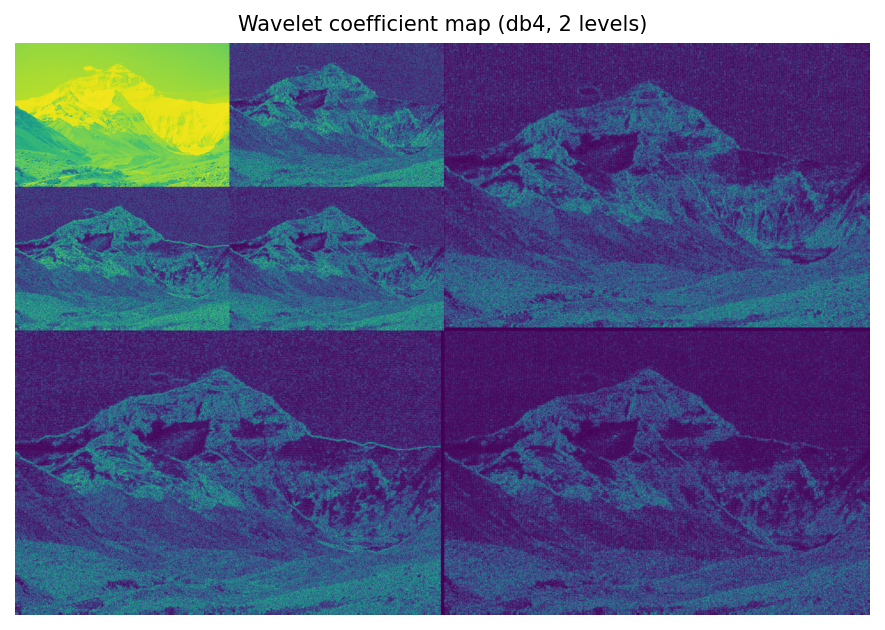
\includegraphics[width=0.6\linewidth]{wavelet_coefficients.png}
  \caption{Wavelet coefficient map (db4, 2 levels, log scale). The
           approximation subband dominates; detail subbands are sparse.}
  \label{fig:wavelet_coeffs}
\end{figure}

\subsection{Quantitative Results}

Tables~\ref{tab:psnr_gaussian} and~\ref{tab:psnr_sp} report PSNR and SSIM for all methods across all three test images.

\begin{table}[H]
\centering
\caption{PSNR (dB) / SSIM under AWGN ($\sigma = 30$)}
\label{tab:psnr_gaussian}
\begin{tabular}{lrrr}
\toprule
Method & PSNR & SSIM \\
\midrule
Noisy input        & 23.88 &  \\
Gaussian filter    & 23.96 & 0.9705 \\
Bilateral filter   & 27.24 & 0.9867 \\
Fourier LP filter  & 23.67 & 0.9688 \\
Wavelet soft (db4) & 22.73 & 0.9608 \\
Median filter      & 26.64 & 0.9843 \\
\bottomrule
\end{tabular}
\end{table}

\begin{table}[H]
\centering
\caption{PSNR (dB) / SSIM under salt-and-pepper noise ($p = 0.05$)}
\label{tab:psnr_sp}
\begin{tabular}{lrrr}
\toprule
Method & PSNR & SSIM \\
\midrule
Noisy input        & 17.86 & \\
Gaussian filter    & 23.54 & 0.9671 \\
Bilateral filter   & 18.53 & 0.9052 \\
Fourier LP filter  & 23.07 & 0.9638 \\
Wavelet soft (db4) & 23.13 & 0.9640 \\
Median filter      & 28.15 & 0.9894 \\
\bottomrule
\end{tabular}
\end{table}

\subsection{Parameter Sensitivity}

\subsubsection{Bilateral Filter: Range Parameter $\sigma_r$}

Table~\ref{tab:bilateral_sweep} shows the effect of varying $\sigma_r$ on the Mountain image under AWGN, with $\sigma_s = 5$ held fixed. Small values of $\sigma_r$ produce under-smoothing because even modest intensity differences suppress the range weight. Large values approach the behavior of a plain Gaussian filter as the range weight tends toward 1 for all neighbors.

\begin{table}[H]
\centering
\caption{Bilateral filter: PSNR and SSIM vs.\ $\sigma_r$ (AWGN, $\sigma=30$, Mountain)}
\label{tab:bilateral_sweep}
\begin{tabular}{crr}
\toprule
$\sigma_r$ & PSNR (dB) & SSIM \\
\midrule
10  & 24.45 & 0.9752 \\
30  & 27.24 & 0.9867 \\
60  & 27.24 & 0.9842 \\
100 & 24.64 & 0.9748\\
\bottomrule
\end{tabular}
\end{table}

\subsubsection{Wavelet: Decomposition Level $L$}

Table~\ref{tab:wavelet_sweep} shows PSNR and SSIM as a function of the number of decomposition levels $L$. Increasing $L$ allows the threshold to be adapted over coarser scales, but can also affect the approximation subband if the image content is not well separated from noise at coarse levels.

\begin{table}[H]
\centering
\caption{Wavelet thresholding: PSNR and SSIM vs.\ decomposition level $L$}
\label{tab:wavelet_sweep}
\begin{tabular}{crr}
\toprule
Level $L$ & PSNR (dB) & SSIM \\
\midrule
1          & 26.11      & 0.9826 \\
2          & 24.04      & 0.9714 \\ 
3          & 22.73      & 0.9608 \\
4          & 22.06      & 0.9537 \\
\bottomrule
\end{tabular}
\end{table}

% ─────────────────────────────────────────────────────────────────────────────
\section{Future Work}

\subsection{Future Work}

Several directions would extend this work. First, the per-pixel loops in the spatial filters are a significant bottleneck; replacing them with vectorized NumPy operations using \texttt{sliding\_window\_view} or a Numba JIT compilation would reduce runtime substantially and make parameter sweeps on full-resolution images tractable.

Second, the Fourier low-pass filter uses a binary (hard) circular mask, which introduces Gibbs ringing at sharp frequency cutoffs. Replacing it with an apodized mask (e.g., Hann window) or a Butterworth frequency response would reduce this artifact.

Third, the bilateral filter could be replaced by the joint bilateral filter or the guided image filter, which offer better edge preservation and significantly lower computational cost.

Finally, extending the evaluation to modern CNN-based denoisers such as DnCNN would provide a reference ceiling on achievable PSNR and SSIM, contextualizing the gap between classical and learning-based methods.

% ─────────────────────────────────────────────────────────────────────────────

\end{document}